\documentclass[12pt,a4paper]{article}
\usepackage[utf8]{inputenc}
\usepackage[vietnamese]{babel}
\usepackage{amsmath,amssymb,amsthm}
\usepackage{geometry,graphicx,booktabs,listings,xcolor,float,fancyhdr,hyperref,titlesec,tcolorbox}
\usepackage{algorithm}\usepackage{algpseudocode}
\usepackage{multirow,caption,subcaption,enumitem}
\tcbuselibrary{skins}
\geometry{left=3cm,right=2cm,top=2.5cm,bottom=2.5cm}
\pagestyle{fancy}\fancyhf{}
\fancyhead[L]{\small\textit{Báo cáo Project Cuối Kỳ — NLP}}
\fancyhead[R]{\small\textit{Nhóm: Hiên -- Đình -- Huyên}}
\fancyfoot[C]{\thepage}\renewcommand{\headrulewidth}{0.4pt}
\lstset{language=Python,basicstyle=\ttfamily\footnotesize,keywordstyle=\color{blue!80!black}\bfseries,
  commentstyle=\color{gray}\itshape,stringstyle=\color{teal},numberstyle=\tiny\color{gray},
  frame=single,rulecolor=\color{gray!40},breaklines=true,numbers=left,xleftmargin=2em,backgroundcolor=\color{gray!5}}
\titleformat{\section}{\large\bfseries\color{blue!70!black}}{{\thesection.}}{0.5em}{}[\vspace{-4pt}\rule{\linewidth}{0.8pt}]
\hypersetup{colorlinks=true,linkcolor=blue!60!black,citecolor=green!50!black}

% ===================================================================
% BẮT ĐẦU TÀI LIỆU
% ===================================================================
\begin{document}

% -------------------------------------------------------------------
% TRANG BÌA
% -------------------------------------------------------------------
\begin{titlepage}\thispagestyle{empty}\newgeometry{left=2.8cm,right=2.8cm,top=2cm,bottom=2cm}
\begin{center}
{\normalsize\bfseries ĐẠI HỌC QUỐC GIA THÀNH PHỐ HỒ CHÍ MINH}\\[2pt]
{\large\bfseries TRƯỜNG ĐẠI HỌC KHOA HỌC TỰ NHIÊN}\\[2pt]
{\normalsize KHOA TOÁN -- TIN HỌC}\vspace{0.6cm}
{\color{black}\rule{\linewidth}{2.5pt}}\\[1pt]{\color{black}\rule{\linewidth}{0.5pt}}\vspace{0.5cm}
{\LARGE\bfseries BÁO CÁO PROJECT CUỐI KỲ}\\[8pt]
{\fontsize{28}{36}\selectfont\bfseries VIETNAMESE GRAPH RAG}\\[6pt]
{\large\bfseries Hệ thống Hỏi đáp Thông minh cho}\\[6pt]
{\large\bfseries Thương mại Điện tử Tiếng Việt}\\[10pt]
{\large\itshape Môn học: Xử Lý Ngôn Ngữ Tự Nhiên (NLP)}\vspace{0.3cm}
{\color{black}\rule{\linewidth}{0.5pt}}\\[1pt]{\color{black}\rule{\linewidth}{2.5pt}}\vspace{1.5cm}
\renewcommand{\arraystretch}{1.6}
\begin{tabular}{r@{\hspace{6pt}:\hspace{10pt}}l}
  {\bfseries Nhóm trưởng}   & Lê Phạm Hồng Hiên -- 22110059 \\[-2pt]
  {\bfseries Thành viên 1}  & Dương Bùi Phương Đình -- 22110049 \\[-2pt]
  {\bfseries Thành viên 2}  & Phạm Xuân Huyên -- 22110076 \\[-2pt]
  {\bfseries Khoa}           & Toán -- Tin học \\[-2pt]
  {\bfseries Giảng viên}     & (Tên giảng viên) \\[-2pt]
  {\bfseries Năm học}        & 2025 -- 2026 \\
\end{tabular}
\vfill{\small Thành phố Hồ Chí Minh, tháng 5 năm 2026}
\end{center}\restoregeometry
\end{titlepage}
\tableofcontents\newpage

% ===================================================================
\section{Giới thiệu}
% ===================================================================

\subsection{Đặt vấn đề}

Thương mại điện tử (TMĐT) tại Việt Nam đang phát triển bùng nổ với các nền tảng như \textbf{Shopee, Lazada, Tiki}. Mỗi ngày, hàng triệu đánh giá sản phẩm được đăng tải, tạo ra nguồn dữ liệu khổng lồ nhưng \textbf{phi cấu trúc}. Người mua hàng thường gặp khó khăn khi tìm kiếm thông tin cụ thể về sản phẩm từ hàng nghìn bình luận --- ví dụ: ``Camera iPhone 15 chụp đêm có tốt không?'' hay ``Pin Samsung S24 dùng được bao lâu?''.

\textbf{Retrieval-Augmented Generation (RAG)} là kiến trúc kết hợp giữa \textit{truy xuất thông tin} (Information Retrieval) và \textit{sinh văn bản} (Text Generation), cho phép mô hình ngôn ngữ trả lời dựa trên \textbf{nguồn tri thức cụ thể} --- ở đây là các đánh giá sản phẩm thực tế.

\textbf{Graph RAG} mở rộng RAG truyền thống bằng cách bổ sung \textbf{đồ thị tri thức (Knowledge Graph)} --- lưu trữ mối quan hệ giữa sản phẩm, thương hiệu, tính năng và cảm xúc người dùng --- giúp truy xuất chính xác và có ngữ cảnh hơn.

\subsection{Mục tiêu dự án}

\begin{enumerate}[leftmargin=2cm]
  \item Xây dựng hệ thống \textbf{Vietnamese Graph RAG} cho bài toán hỏi đáp về sản phẩm TMĐT.
  \item \textbf{So sánh} các phương pháp biểu diễn văn bản: TF-IDF, Word2Vec, GloVe, PhoBERT; có thêm subword (BPE) và mô hình tuần tự \textbf{BiLSTM}.
  \item \textbf{Trích xuất thực thể} (NER) và \textbf{phân loại aspect} bằng BiLSTM từ đánh giá.
  \item Xây dựng \textbf{Knowledge Graph} thể hiện quan hệ sản phẩm -- thuộc tính -- cảm xúc.
  \item \textbf{Đánh giá} hiệu quả Graph RAG (ablation Bi-encoder / Attention / Graph).
  \item \textbf{Đóng gói LLMOps}: serving API, observability, vòng lặp train$\to$deploy mô hình.
\end{enumerate}

\subsection{Phạm vi}

\begin{itemize}[leftmargin=2cm]
  \item \textbf{Domain}: Thương mại điện tử --- đánh giá sản phẩm tiếng Việt (smartphone + đa sản phẩm)
  \item \textbf{Dataset}: \textbf{(1)} UIT-ViSFD --- 11,122 review smartphone, 10 aspect (train 7,786 dùng thực nghiệm); \textbf{(2)} Shopee reviews --- 3,154 review đa sản phẩm (26 sản phẩm, 24 shop) có \texttt{product/shop/rating}. Tổng corpus truy xuất $\approx$ 10,9k review.
  \item \textbf{Mô hình}: TF-IDF, Word2Vec, GloVe-SVD (Lec02); Subword/BPE (Lec03); BiLSTM (Lec05); PhoBERT + Attention/MaxSim (Lec06)
  \item \textbf{LLM}: OpenAI API (gpt-4o-mini) cho phần Generation
  \item \textbf{Triển khai}: pipeline LLMOps (FastAPI + Gradio + observability + CI/Docker), có vòng lặp train$\to$deploy mô hình BiLSTM
\end{itemize}

% ===================================================================
\section{Cơ sở lý thuyết}
% ===================================================================

\subsection{Tiền xử lý văn bản tiếng Việt}

Tiếng Việt là ngôn ngữ \textbf{đơn lập} (isolating language), trong đó ranh giới từ không được xác định bằng khoảng trắng. Ví dụ: ``học sinh'' là một từ ghép, không phải hai từ riêng biệt.

\textbf{Công cụ sử dụng}: Thư viện \texttt{underthesea} cung cấp chức năng tách từ (word segmentation) cho tiếng Việt:

\begin{lstlisting}[caption={Tách từ tiếng Việt}]
from underthesea import word_tokenize
text = "Truong Dai hoc Khoa hoc Tu nhien"
tokens = word_tokenize(text, format="text")
# "Truong_Dai_hoc Khoa_hoc Tu_nhien"
\end{lstlisting}

\subsection{Bag of Words và TF-IDF}

\textbf{TF-IDF} (Term Frequency -- Inverse Document Frequency) đo lường mức độ quan trọng của một từ trong tài liệu so với toàn bộ tập tài liệu:
\[
  \text{TF-IDF}(t, d) = \text{TF}(t, d) \times \log\frac{N}{1 + \text{DF}(t)}
\]

Trong dự án, TF-IDF được sử dụng làm \textbf{baseline} cho việc truy xuất đánh giá sản phẩm liên quan đến câu hỏi của người dùng.

\subsection{Word Embeddings: Word2Vec và GloVe}

\textbf{Word2Vec} (Mikolov et al., 2013) học biểu diễn từ dựa trên \textit{ngữ cảnh lân cận}:
\begin{itemize}
  \item \textbf{Skip-gram}: Dự đoán từ ngữ cảnh từ từ trung tâm
  \item \textbf{CBOW}: Dự đoán từ trung tâm từ ngữ cảnh
\end{itemize}

\textbf{GloVe} (Pennington et al., 2014) học embeddings dựa trên \textit{ma trận đồng xuất hiện}, tối ưu hàm mất mát:
\[
  J = \sum_{i,j} f(X_{ij}) \left( w_i^T w_j + b_i + b_j - \log X_{ij} \right)^2
\]

\subsection{Mô hình Subword (BPE)}

Các embedding ở trên giả định một \textbf{từ vựng cố định}, nên khi gặp \textbf{từ hiếm hoặc ngoài từ vựng (OOV)} sẽ không có vector biểu diễn. \textbf{Byte-Pair Encoding (BPE)} khắc phục bằng cách tách từ thành các \textbf{mảnh con (subword)} xuất hiện thường xuyên --- ví dụ ``chống\_nước'' $\to$ [``chống'', ``\_nước'']. Nhờ vậy mọi từ đều biểu diễn được qua tổ hợp subword, kể cả từ chưa từng thấy khi huấn luyện. PhoBERT sử dụng BPE trên dữ liệu tiếng Việt đã tách từ.

\subsection{Mạng nơ-ron hồi quy (RNN / LSTM)}

RNN xử lý dữ liệu \textbf{tuần tự} bằng trạng thái ẩn truyền qua từng bước thời gian: $h_t = f(h_{t-1}, x_t)$. \textbf{LSTM} bổ sung các cổng (input/forget/output) để giảm hiện tượng \textit{vanishing gradient} và nắm bắt phụ thuộc xa. \textbf{BiLSTM} đọc chuỗi theo cả hai chiều rồi ghép biểu diễn, phù hợp cho bài toán phân loại câu. Trong dự án, BiLSTM được dùng để phân loại đa nhãn aspect (Mục~\ref{sec:rnn}).

\subsection{Transformer và BERT/PhoBERT}

\textbf{Transformer} (Vaswani et al., 2017) sử dụng cơ chế \textbf{Self-Attention} để xử lý song song toàn bộ chuỗi:
\[
  \text{Attention}(Q, K, V) = \text{softmax}\left(\frac{QK^T}{\sqrt{d_k}}\right) V
\]

\textbf{PhoBERT} (Nguyen \& Nguyen, 2020) là mô hình BERT được pre-train trên 20GB dữ liệu tiếng Việt, đạt state-of-the-art trên nhiều tác vụ NLP tiếng Việt.

\subsection{Retrieval-Augmented Generation (RAG)}

RAG kết hợp hai thành phần:
\begin{enumerate}
  \item \textbf{Retriever}: Tìm kiếm tài liệu liên quan từ knowledge base
  \item \textbf{Generator}: Sinh câu trả lời dựa trên tài liệu đã tìm được
\end{enumerate}

\subsection{Knowledge Graph và Graph RAG}

Knowledge Graph lưu trữ thông tin dưới dạng \textbf{bộ ba} (triple): $(h, r, t)$ --- head entity, relation, tail entity. Ví dụ trong TMĐT:

\begin{center}
\texttt{(iPhone\_15, thuộc\_thương\_hiệu, Apple)} \\
\texttt{(iPhone\_15, có\_tính\_năng, Camera\_48MP)} \\
\texttt{(Camera\_48MP, được\_đánh\_giá, Tích\_cực\_85\%)}
\end{center}

Graph RAG bổ sung bước \textbf{graph traversal} vào pipeline RAG, cho phép truy xuất thông tin có cấu trúc --- ví dụ khi hỏi về ``camera iPhone 15'', hệ thống có thể duyệt graph để tìm tất cả đánh giá liên quan đến tính năng camera.

% ===================================================================
\section{Dataset và Tiền xử lý dữ liệu}
% ===================================================================

\subsection{Dataset sử dụng}

\begin{table}[H]
\centering
\caption{Tổng hợp các dataset sử dụng trong dự án}
\begin{tabular}{llrl}
\toprule
\textbf{Dataset} & \textbf{Tác vụ} & \textbf{Kích thước} & \textbf{Nguồn} \\
\midrule
UIT-ViSFD & Aspect-Based Sentiment & 11,122 comments & Shopee \\
Shopee reviews & Review đa sản phẩm & 3,154 reviews & GitHub (nhtlongcs) \\
PhoNER\_COVID19 & NER (tham khảo) & domain COVID & HuggingFace \\
\bottomrule
\end{tabular}
\\[4pt]
{\small\textit{Ghi chú: PhoNER\_COVID19 thuộc domain COVID nên không phù hợp gán nhãn thực thể sản phẩm; chỉ tải về tham khảo. Việc trích xuất thương hiệu dùng NER tổng quát (\texttt{underthesea}) kết hợp gazetteer.}}
\end{table}

\subsection{Dataset chính: UIT-ViSFD}

\textbf{UIT-ViSFD} (Vietnamese Smartphone Feedback Dataset) là bộ dữ liệu đánh giá smartphone từ sàn TMĐT Việt Nam, được gán nhãn bởi con người với:

\begin{itemize}
  \item \textbf{10 aspect categories}: SCREEN, CAMERA, BATTERY, PERFORMANCE, STORAGE, DESIGN, PRICE, GENERAL, FEATURES, SER\&ACC (Service \& Accessories)
  \item \textbf{3 sentiment polarities}: Positive, Negative, Neutral
  \item \textbf{11,122 comments} với annotation ở mức aspect-level
\end{itemize}

\textbf{Ví dụ dữ liệu}:
\begin{quote}
\textit{``Camera chụp đêm rất nét, pin dùng được 2 ngày, nhưng giá hơi cao so với cấu hình.''}\\
$\rightarrow$ CAMERA: Positive, BATTERY: Positive, PRICE: Negative
\end{quote}

\begin{lstlisting}[caption={Tải và parse nhãn UIT-ViSFD (đúng định dạng thực tế)}]
import pandas as pd, re
df = pd.read_csv("data/raw/Train.csv")   # cot: index, comment, n_star, label
# nhan co dang: "{CAMERA#Positive};{SER&ACC#Negative};{OTHERS};"
PAT = re.compile(r"\{([\w&]+)#(\w+)\}")   # giu '&' de KHONG mat aspect SER&ACC
def parse_label(s):
    if pd.isna(s): return []
    return [(m.group(1), m.group(2)) for m in PAT.finditer(str(s))]
df["aspects"] = df["label"].apply(lambda s: [a for a, _ in parse_label(s)])
print(f"Total: {len(df)} | vi du nhan: {df['label'].iloc[0]}")
\end{lstlisting}

\subsection{Dataset bổ sung: Shopee reviews}

Để mở rộng ngoài domain smartphone, chúng tôi bổ sung \textbf{3.154 review Shopee đa sản phẩm} (26 sản phẩm, 24 shop) gồm các trường \texttt{comment, product\_name, shop\_name, rating\_star}. Bộ này \textbf{không có nhãn aspect}, nên được dùng cho hai mục đích: (1) mở rộng corpus truy xuất (Graph RAG trả lời được câu hỏi đa sản phẩm), và (2) cung cấp các thực thể \texttt{shop}/\texttt{product} cho Knowledge Graph. Aspect cho review Shopee được \textbf{dự đoán bằng mô hình BiLSTM} (Mục~\ref{sec:rnn}) thay vì nhãn vàng.

\subsection{Phân tích nhãn aspect}

Nhãn của UIT-ViSFD có dạng chuỗi \texttt{\{ASPECT\#Sentiment\}} ngăn cách bởi dấu \texttt{;}. Một điểm cần lưu ý: aspect \textbf{SER\&ACC} chứa ký tự \texttt{\&}, nên biểu thức chính quy ngây thơ \texttt{\textbackslash\{(\textbackslash w+)\#(\textbackslash w+)\textbackslash\}} sẽ \textbf{bỏ sót} aspect này (1.995 lần trong tập train --- aspect phổ biến thứ 7). Chúng tôi sửa thành \texttt{\textbackslash\{([\textbackslash w\&]+)\#(\textbackslash w+)\textbackslash\}} để giữ đủ 10 aspect.

\subsection{Pipeline tiền xử lý}

\begin{enumerate}
  \item \textbf{Cleaning}: lowercase, loại URL, ký tự đặc biệt, chữ số, chuẩn hóa khoảng trắng.
  \item \textbf{Word Segmentation}: tách từ tiếng Việt bằng \texttt{underthesea}.
  \item \textbf{Stopword Removal}: loại từ dừng (cho TF-IDF/Word2Vec/GloVe).
  \item \textbf{Lưu ý nhất quán}: PhoBERT dùng văn bản \textbf{đã tách từ nhưng giữ dấu/số} (không loại stopword), đúng với pipeline khuyến nghị của PhoBERT; các phương pháp đếm dùng bản đã làm sạch.
\end{enumerate}

% ===================================================================
\section{Kiến trúc hệ thống}
% ===================================================================

\subsection{Tổng quan Pipeline}

\begin{figure}[H]
  \centering
  \includegraphics[width=0.95\textwidth]{figures/architecture.png}
  \caption{Kiến trúc tổng quan hệ thống Vietnamese Graph RAG gồm 6 module chính}
  \label{fig:architecture}
\end{figure}

\begin{figure}[H]
  \centering
  \includegraphics[width=0.9\textwidth]{figures/sequence_diagram.png}
  \caption{Sequence Diagram: Luồng xử lý khi người dùng đặt câu hỏi}
  \label{fig:sequence}
\end{figure}

Hệ thống gồm 6 module chính:

\begin{enumerate}
  \item \textbf{Module 1 -- Tiền xử lý}: Xử lý văn bản tiếng Việt (tách từ, loại stopwords)
  \item \textbf{Module 2 -- Embedding}: So sánh TF-IDF, Word2Vec, GloVe, PhoBERT
  \item \textbf{Module 3 -- NER}: Trích xuất thực thể bằng underthesea + gazetteer
  \item \textbf{Module 4 -- Knowledge Graph}: Xây dựng đồ thị tri thức (NetworkX)
  \item \textbf{Module 5 -- Retrieval}: Embedding + Graph boost + Attention (MaxSim) re-ranking
  \item \textbf{Module 6 -- Generation}: Tích hợp LLM API (OpenAI)
\end{enumerate}

\subsection{Bám sát chương trình môn học (6 lecture)}

Các thành phần của hệ thống ánh xạ trực tiếp tới 6 bài giảng của môn:

\begin{table}[H]
\centering
\renewcommand{\arraystretch}{1.25}
\begin{tabular}{p{3.4cm}p{4.2cm}p{5.2cm}}
\toprule
\textbf{Lecture} & \textbf{Nội dung} & \textbf{Áp dụng trong project} \\
\midrule
Lec02 -- Word Representation & one-hot, TF-IDF, Word2Vec, GloVe & So sánh TF-IDF / Word2Vec / GloVe-SVD \\
Lec03 -- Subword Models & BPE, subword & Tokenize BPE (PhoBERT) cho từ hiếm/OOV \\
Lec04 -- Compositional Semantics & Document$\to$Sentence$\to$Phrase$\to$Word & Knowledge Graph: brand$\to$aspect$\to$sentiment, shop$\to$product \\
Lec05 -- Recurrent Neural Networks & RNN/LSTM, dữ liệu tuần tự & BiLSTM phân loại đa nhãn aspect (micro-F1) \\
Lec06 -- Attention \& Transformer & attention, encoder--decoder & PhoBERT + tái xếp hạng MaxSim (late-interaction) \\
\bottomrule
\end{tabular}
\caption{Ánh xạ thành phần hệ thống $\leftrightarrow$ 6 lecture của môn.}
\end{table}

\subsection{Module 1: Tiền xử lý}

Chuẩn hoá văn bản tiếng Việt: lowercase, loại URL/ký tự đặc biệt/chữ số, \textbf{tách từ} bằng \texttt{underthesea}, loại stopword (cho nhóm phương pháp đếm). PhoBERT dùng bản \textit{đã tách từ nhưng giữ dấu/số}. Toàn bộ gói trong hàm \texttt{preprocess\_vietnamese} --- \textbf{dùng chung} cho cả huấn luyện BiLSTM lẫn suy luận để đảm bảo nhất quán từ vựng (chi tiết ở Mục~3.5).

\subsection{Module 2: So sánh Embedding Methods}

Đây là module quan trọng nhất, thể hiện kiến thức NLP cốt lõi. Chúng tôi so sánh 4 phương pháp biểu diễn văn bản:

\begin{table}[H]
\centering
\caption{So sánh 4 phương pháp Embedding}
\begin{tabular}{llll}
\toprule
\textbf{Phương pháp} & \textbf{Loại} & \textbf{Đặc điểm} & \textbf{Lecture} \\
\midrule
TF-IDF & Sparse, thống kê & Baseline, không capture ngữ nghĩa & Lec02 \\
Word2Vec & Dense, predictive & Skip-gram/CBOW, ngữ cảnh cục bộ & Lec02 \\
GloVe & Dense, count-based & Co-occurrence matrix, ngữ nghĩa toàn cục & Lec02 \\
PhoBERT & Dense, contextual & Transformer, tiếng Việt, SOTA & Lec06 \\
\bottomrule
\end{tabular}
\end{table}

\begin{figure}[H]
  \centering
  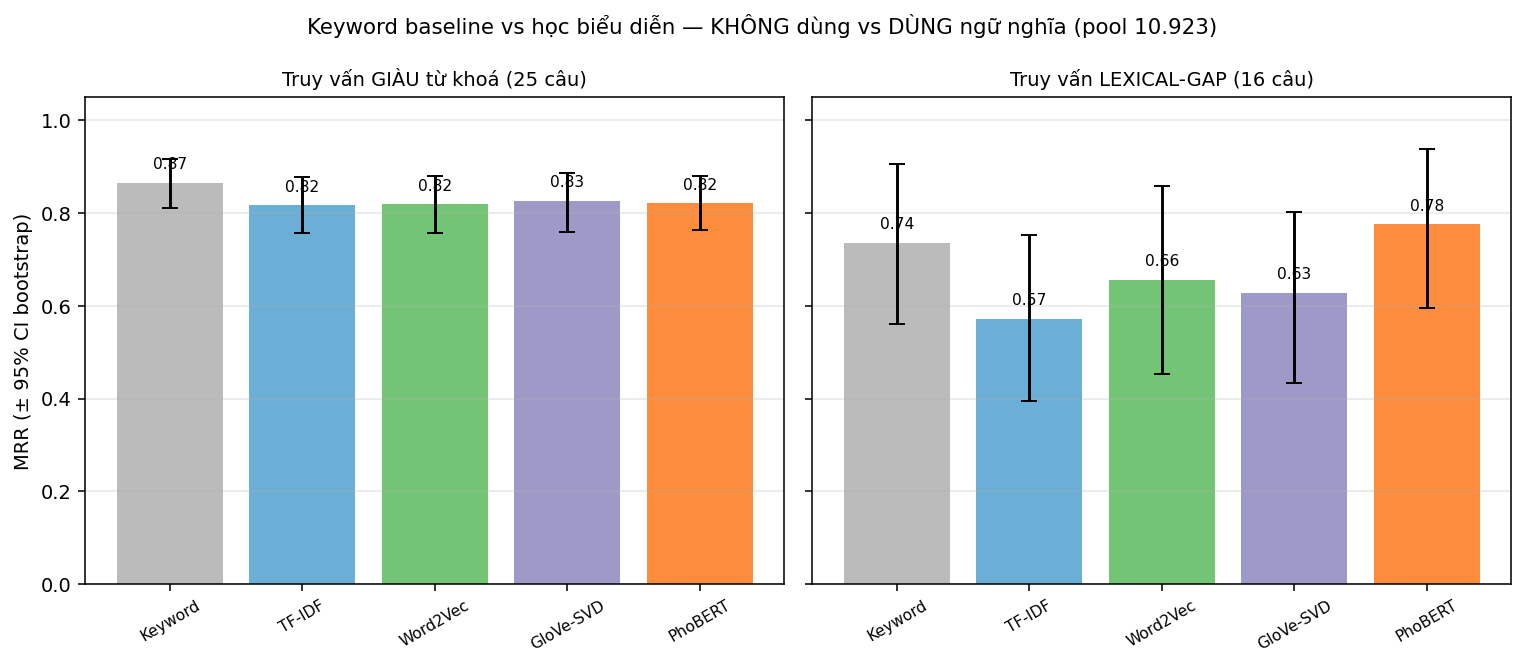
\includegraphics[width=0.85\textwidth]{figures/embedding_comparison.png}
  \caption{So sánh hiệu quả Retrieval giữa 4 phương pháp Embedding (Precision@k \& MRR)}
  \label{fig:embedding_comparison}
\end{figure}

\textbf{Lưu ý về độ đo}: không dùng ``trung bình cosine similarity'' để so sánh, vì độ lớn cosine \textbf{không so sánh được} giữa các không gian embedding khác nhau (TF-IDF thưa cho giá trị thấp hơn PhoBERT dày). Thay vào đó dùng \textbf{Precision@k} và \textbf{MRR} với ground-truth là nhãn aspect (xem Mục~\ref{sec:exp1}).

\textbf{Lưu ý về ``GloVe''}: do hạn chế tài nguyên, chúng tôi dùng \textbf{xấp xỉ kiểu GloVe} --- SVD trên ma trận đồng xuất hiện ở mức tài liệu (gần với LSA), không phải GloVe cửa sổ ngữ cảnh gốc.

\subsection{Module 3: Named Entity Recognition}

NER tổng quát của \texttt{underthesea} (nhãn PER/LOC/ORG) bắt tốt các thực thể \textbf{thương hiệu} và \textbf{cửa hàng} (vd. \textit{Apple}, \textit{Thế Giới Di Động}). Thực thể đặc thù e-commerce (dòng máy) không nằm trong tập nhãn tổng quát nên được bổ sung bằng \textbf{gazetteer thương hiệu}. Các thực thể thương hiệu này được đưa vào Knowledge Graph làm node \texttt{brand}. (PhoNER\_COVID19 không dùng vì khác domain.)

\subsection{Module 4: Knowledge Graph}

\begin{figure}[H]
  \centering
  \IfFileExists{figures/knowledge_graph.png}{%
    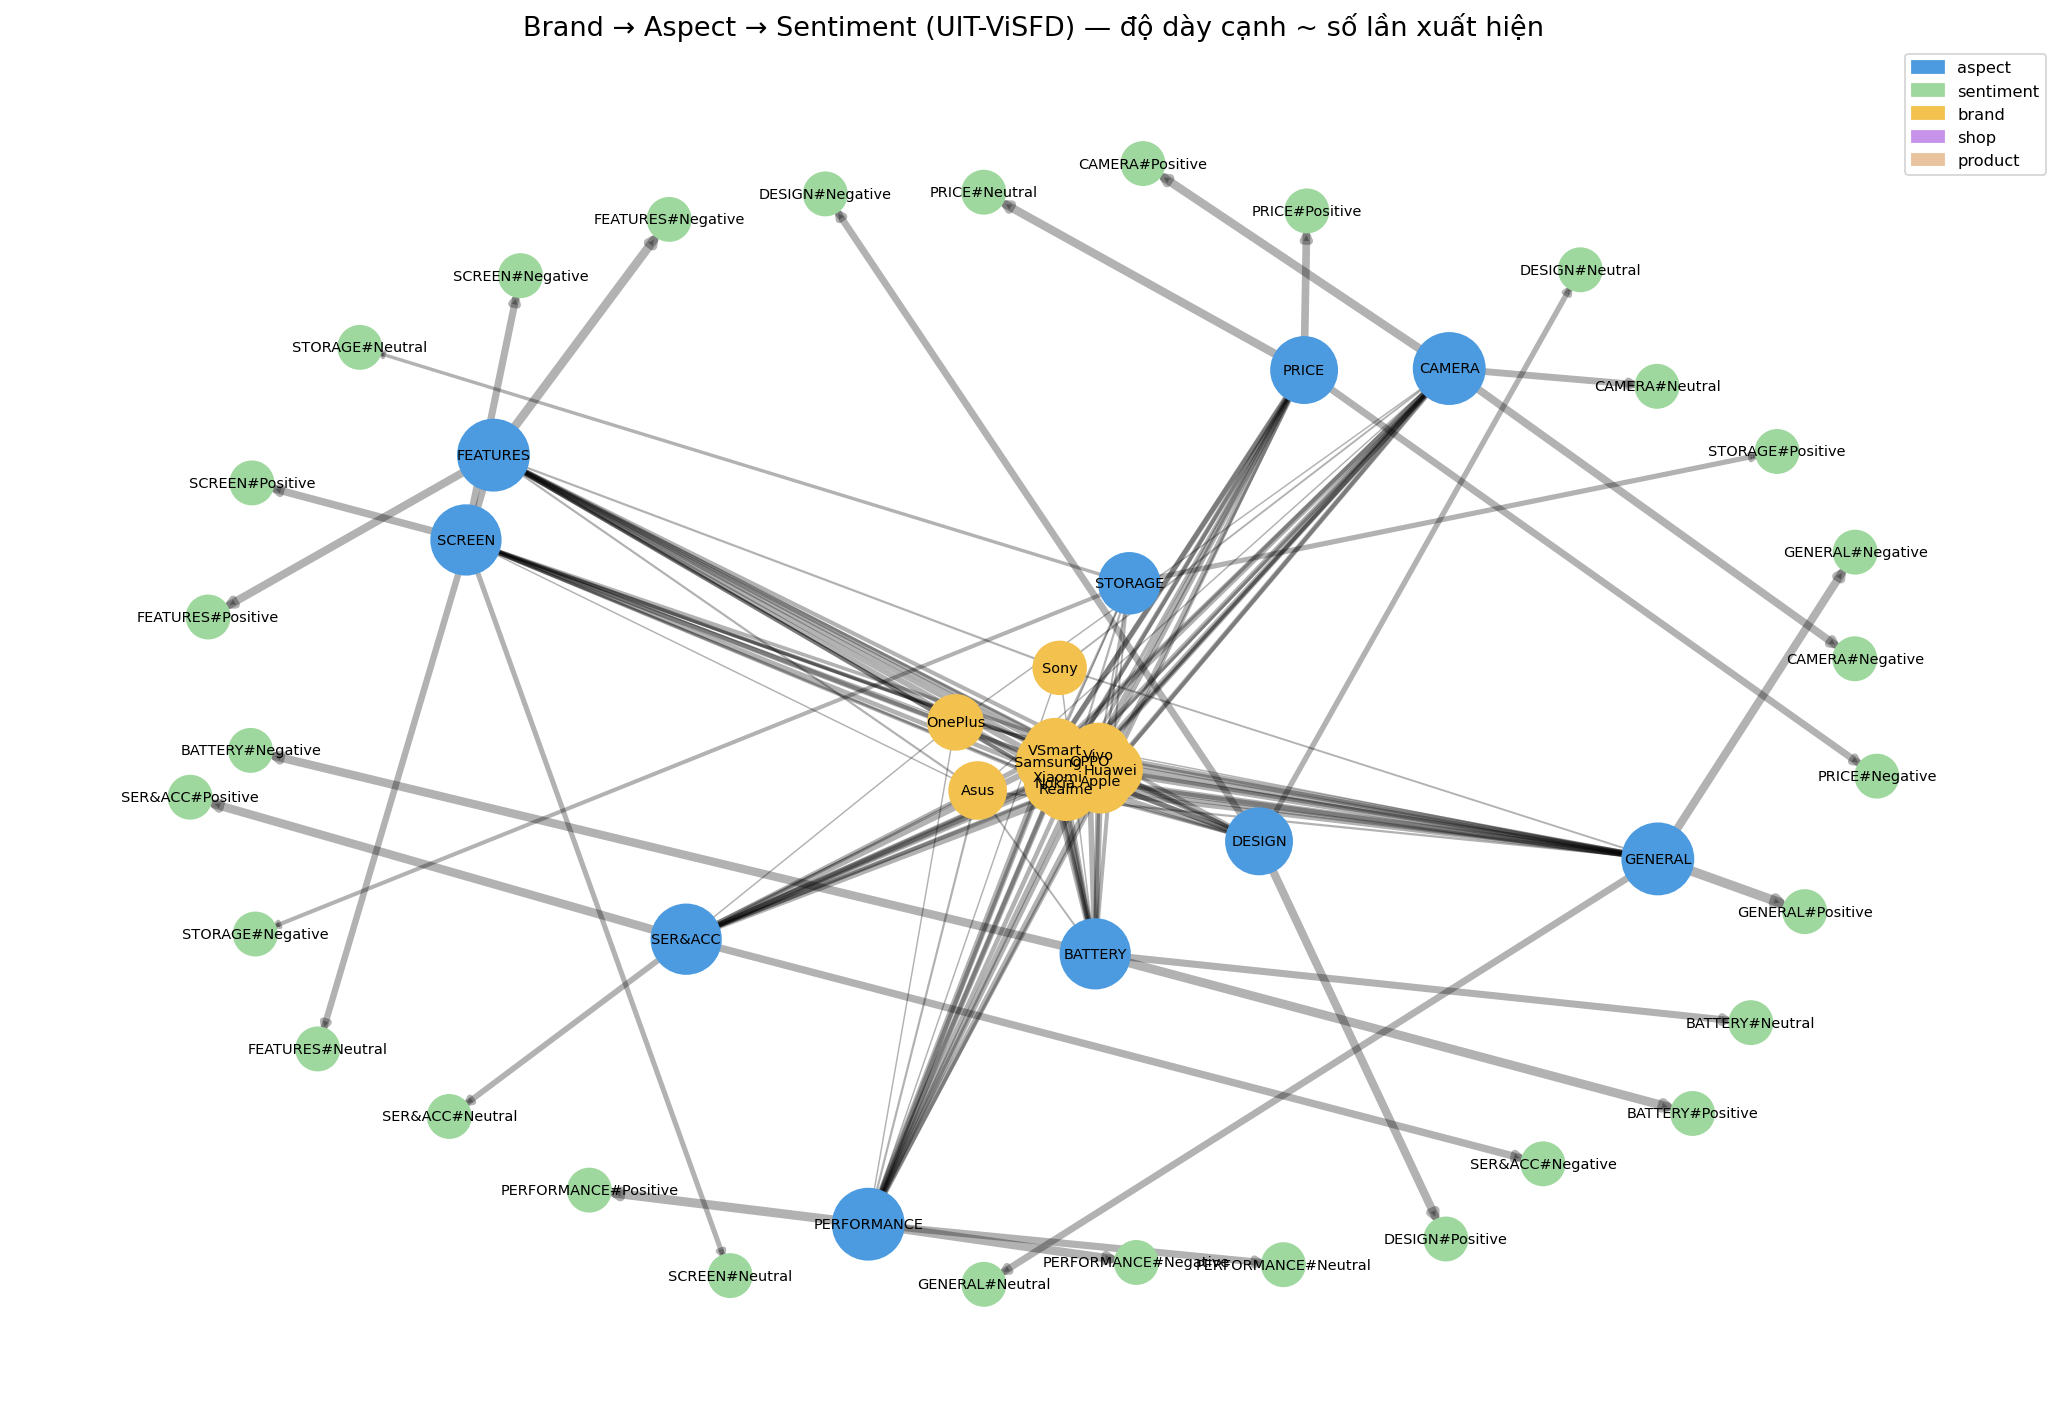
\includegraphics[width=0.9\textwidth]{figures/knowledge_graph.png}}{%
    \fbox{\parbox{0.8\textwidth}{\centering\textit{Copy \texttt{fig\_knowledge\_graph.png} từ output notebook Part 2 vào \texttt{report/figures/knowledge\_graph.png}}}}}
  \caption{Knowledge Graph: \texttt{brand} $\to$ \texttt{aspect} $\to$ \texttt{aspect\#sentiment}, trọng số cạnh = số review.}
  \label{fig:kg}
\end{figure}

Đồ thị có hướng (NetworkX) gồm 3 loại node: \texttt{brand}, \texttt{aspect} (10 aspect gồm SER\&ACC) và \texttt{aspect\#sentiment}. Cạnh \texttt{brand}$\to$\texttt{aspect} và \texttt{aspect}$\to$\texttt{sentiment} mang trọng số là số review, cho phép truy vấn phân bố cảm xúc theo từng khía cạnh.

\subsection{Module 5: Retrieval với Attention Re-ranking}

Pipeline truy xuất 2 tầng: (1) \textbf{bi-encoder} PhoBERT (mean-pooling) tính cosine để lấy Top-50 candidate; (2) \textbf{tái xếp hạng late-interaction (MaxSim, kiểu ColBERT)} --- với mỗi token của truy vấn, lấy cosine lớn nhất so với các token của tài liệu rồi tính trung bình. Đây là cơ chế \textbf{attention} (tích vô hướng có chuẩn hoá giữa token query và token doc), \textbf{không tham số ngẫu nhiên và không cần huấn luyện}. Điểm cuối kết hợp: bi-encoder, MaxSim, và một \textbf{graph boost} dựa trên aspect quan sát được trong nội dung review.

\subsection{Module 6: Generation (OpenAI)}

Ghép Top-$k$ review truy xuất và thống kê từ Knowledge Graph thành một prompt có \textbf{grounding} (chỉ trả lời dựa trên dữ liệu cung cấp), rồi gọi \textbf{OpenAI} (\texttt{gpt-4o-mini}, temperature 0.3) sinh câu trả lời tiếng Việt. Khi thiếu API key, hệ thống \textbf{fallback} trả về các review truy xuất thay vì lỗi. Mỗi lần gọi được ghi log latency + token + chi phí USD (Mục~\ref{sec:llmops}).

% ===================================================================
\section{Thực nghiệm}
% ===================================================================

\subsection{Môi trường thực nghiệm}

\begin{table}[H]
\centering
\caption{Cấu hình môi trường thực nghiệm}
\begin{tabular}{ll}
\toprule
\textbf{Thành phần} & \textbf{Chi tiết} \\
\midrule
Platform & Kaggle Notebook (T4 GPU) \\
Python & 3.10+ \\
PyTorch & 2.x \\
Transformers & 4.40+ \\
LLM & OpenAI API (gpt-4o-mini) \\
Các thư viện khác & underthesea, gensim, networkx, openai, gradio \\
\bottomrule
\end{tabular}
\end{table}

\subsection{Thí nghiệm 1: So sánh Embedding Methods}
\label{sec:exp1}

\textbf{Thiết lập}: 9 truy vấn (mỗi truy vấn nhắm 1 aspect). Một review được coi là \textit{liên quan} nếu nhãn vàng của nó chứa aspect đó. Báo cáo Precision@5, Precision@10, MRR (trung bình trên các truy vấn). Cùng một phán quyết liên quan áp dụng cho cả 4 phương pháp $\Rightarrow$ công bằng.

\begin{table}[H]
\centering
\caption{Precision@k \& MRR theo phương pháp embedding \textit{(điền số từ \texttt{results\_part1.json} / bảng LaTeX in ra ở notebook Part 1)}}
\begin{tabular}{lrrr}
\toprule
\textbf{Phương pháp} & \textbf{P@5} & \textbf{P@10} & \textbf{MRR} \\
\midrule
TF-IDF     & \dots & \dots & \dots \\
Word2Vec   & \dots & \dots & \dots \\
GloVe-SVD  & \dots & \dots & \dots \\
PhoBERT    & \dots & \dots & \dots \\
\bottomrule
\end{tabular}
\end{table}

\subsection{Thí nghiệm 2: Trích xuất thực thể (NER)}

Thống kê số thực thể theo loại (PER/LOC/ORG + BRAND từ gazetteer) trên 800 review mẫu được in ở notebook Part 1 (\texttt{results\_part1.json}). Phân tích định tính: NER tổng quát nhận diện tốt thương hiệu (ORG) và địa điểm cửa hàng (LOC); gazetteer bổ sung node \texttt{brand} cho KG.

\subsection{Thí nghiệm 2b: Phân loại aspect bằng RNN (BiLSTM)}
\label{sec:rnn}

Hiện thực \textbf{Lec05 (Recurrent Neural Networks)}: một \textbf{BiLSTM} (embedding 100, hidden 128, hai chiều) phân loại \textbf{đa nhãn} 10 aspect từ review, huấn luyện trên tập train UIT-ViSFD và đánh giá \textbf{micro-F1} trên tập dev. Mô hình sau khi train được \textbf{lưu lại} (\texttt{artifacts/aspect\_clf.pt}) và \textbf{triển khai} trong hệ thống (xem Mục~\ref{sec:llmops}): dùng để gán aspect cho review Shopee (không có nhãn) nhằm làm giàu Knowledge Graph, và phục vụ trực tiếp qua API \texttt{POST /classify}.

\begin{center}
\textit{Micro-F1 (dev): \textbf{[điền từ results\_part1.json / artifacts/metrics.json]}}
\end{center}

\subsection{Thí nghiệm 3: Ablation chiến lược Retrieval (không rò rỉ metric)}

\textbf{Thiết lập}: trên cùng tập Top-50 candidate, thay đổi trọng số 3 thành phần. \textbf{Quan trọng}: graph boost dựa trên aspect \textit{quan sát trong nội dung review} (tín hiệu khả dụng lúc suy luận), còn phán quyết liên quan dùng \textit{nhãn vàng} --- hai nguồn độc lập nên không có rò rỉ.

\begin{table}[H]
\centering
\caption{Ablation: đóng góp của Attention và Graph \textit{(điền từ \texttt{results\_part2.json})}}
\begin{tabular}{lrrr}
\toprule
\textbf{Cấu hình} & \textbf{P@5} & \textbf{P@10} & \textbf{MRR} \\
\midrule
Bi-encoder (PhoBERT) & \dots & \dots & \dots \\
\quad + Attention rerank (MaxSim) & \dots & \dots & \dots \\
\quad + Graph (Graph RAG) & \dots & \dots & \dots \\
\bottomrule
\end{tabular}
\end{table}

\subsection{Thí nghiệm 4: Demo End-to-End}

Ba câu hỏi mẫu (camera, pin, dịch vụ/bảo hành) chạy qua pipeline đầy đủ Retrieve $\to$ Graph context $\to$ OpenAI (gpt-4o-mini). Câu trả lời mẫu và thống kê KG kèm theo được in ở notebook Part 2.

% ===================================================================
\section{Kết quả và Thảo luận}
% ===================================================================

\textbf{Embedding}: kỳ vọng PhoBERT đạt P@k/MRR cao nhất nhờ biểu diễn ngữ cảnh, TF-IDF là baseline; Word2Vec/GloVe-SVD ở giữa. Số liệu cụ thể điền từ Thí nghiệm 1.

\textbf{Retrieval}: ablation cho thấy đóng góp riêng của (i) tái xếp hạng attention MaxSim và (ii) graph boost. Vì đánh giá không còn rò rỉ metric (boost từ nội dung, chấm điểm bằng nhãn vàng), chênh lệch quan sát được phản ánh cải thiện thực --- không còn là kết quả ``được sắp đặt'' như cách boost trực tiếp theo nhãn vàng.

\textbf{Hạn chế quan sát được}: graph boost chỉ kích hoạt khi câu hỏi khớp được aspect tiếng Việt; với câu hỏi mơ hồ (không nêu rõ khía cạnh), đóng góp của graph giảm.

% ===================================================================
\section{Triển khai LLMOps}
\label{sec:llmops}
% ===================================================================

Ngoài notebook khám phá, hệ thống được đóng gói thành một \textbf{pipeline LLMOps production-lite} (package \texttt{src/vngraphrag}) tách hai pha:

\begin{itemize}
  \item \textbf{Offline (build)}: encode corpus bằng PhoBERT, dựng index + Knowledge Graph, lưu thành \textit{artifacts có version} (\texttt{doc\_vectors.npy}, \texttt{records.json}, \texttt{manifest.json}, \texttt{kg.pkl}). Manifest gắn mã version = hash(model, số bản ghi) để chặn việc nạp nhầm index cũ.
  \item \textbf{Online (serve)}: nạp lại artifacts; mỗi truy vấn đi qua \texttt{retrieve $\to$ graph context $\to$ generate} và được ghi log đo đạc.
\end{itemize}

\begin{table}[H]
\centering
\renewcommand{\arraystretch}{1.25}
\begin{tabular}{p{4.2cm}p{8.5cm}}
\toprule
\textbf{Thành phần LLMOps} & \textbf{Hiện thực} \\
\midrule
Cấu hình \& secret & \texttt{config.yaml} + biến môi trường (\texttt{OPENAI\_API\_KEY} chỉ qua env) \\
Versioning artifact & \texttt{DocumentIndex} manifest; tự rebuild khi model/dữ liệu đổi \\
\textbf{Train $\to$ deploy model} & BiLSTM train ở notebook §6 \textbf{hoặc} CLI \texttt{make train} $\to$ \texttt{aspect\_clf.pt} $\to$ nạp ở \texttt{core/aspect\_clf.py} $\to$ phục vụ qua \texttt{POST /classify}; đồng thời gán aspect cho review Shopee để làm giàu KG \\
Serving API & FastAPI: \texttt{/query}, \texttt{/classify}, \texttt{/feedback}, \texttt{/health} \\
Giao diện + feedback loop & Gradio UI, nút thích/không-thích $\to$ \texttt{logs/feedback.jsonl} \\
Observability & mỗi truy vấn log latency + token + \textbf{chi phí USD} vào \texttt{logs/queries.jsonl} \\
Đánh giá + regression gate & \texttt{evaluate.py}: Precision@k/MRR (retrieval) và micro-F1 (BiLSTM); CI fail nếu tụt dưới ngưỡng \\
Đóng gói + CI & \texttt{Dockerfile} + GitHub Actions (lint + test) \\
\bottomrule
\end{tabular}
\caption{Các thành phần LLMOps của hệ thống.}
\end{table}

Điểm đáng chú ý là \textbf{vòng lặp train $\to$ deploy} khép kín: mô hình BiLSTM (Lec05) huấn luyện trong notebook được lưu thành artifact, nạp lại bởi package phục vụ, và sử dụng thực sự ở hai nơi --- gán aspect cho dữ liệu Shopee chưa nhãn (làm giàu Knowledge Graph) và phục vụ trực tiếp qua endpoint \texttt{/classify}.

% ===================================================================
\section{Phân công công việc}
% ===================================================================

\begin{table}[H]
\centering
\caption{Phân công công việc nhóm}
\renewcommand{\arraystretch}{1.4}
\begin{tabular}{p{4cm}p{4.5cm}p{4.5cm}}
\toprule
\textbf{Lê Phạm Hồng Hiên} \newline 22110059 \newline \textit{} 
& \textbf{Dương Bùi Phương Đình} \newline 22110049
& \textbf{Phạm Xuân Huyên} \newline 22110076 \\
\midrule
Kiến trúc tổng thể & Tiền xử lý dữ liệu (Lec01) & Word Representation (Lec02) \\
Module 5: Attention/MaxSim re-ranking (Lec06) & Module 1: Preprocessing & Module 2: So sánh embedding (P@k/MRR) \\
Module 6: RAG Pipeline + OpenAI & Module 3: NER + gazetteer & Subword/BPE (Lec03) \\
\textbf{LLMOps}: package, FastAPI, CI/Docker, observability & \textbf{RNN/BiLSTM (Lec05)}: train + deploy aspect classifier & Module 4: Knowledge Graph + Gradio UI \\
Tích hợp \& testing (\texttt{make check}) & Tích hợp dataset \textbf{Shopee} & Evaluation \& metrics (gate) \\
Báo cáo \& trình bày & Báo cáo (Data, NER, RNN) & Báo cáo (Embedding, KG) \\
\bottomrule
\end{tabular}
\end{table}

% ===================================================================
\section{Kết luận}
% ===================================================================

\subsection{Tóm tắt kết quả}
Dự án xây dựng pipeline Graph RAG hoàn chỉnh cho đánh giá sản phẩm tiếng Việt trên \textbf{hai dataset} (UIT-ViSFD smartphone + Shopee đa sản phẩm). Hệ thống phủ trọn 6 lecture của môn: biểu diễn từ (TF-IDF/Word2Vec/GloVe), subword/BPE, ngữ nghĩa tổ hợp (Knowledge Graph), BiLSTM (phân loại aspect), và Transformer/attention (PhoBERT + MaxSim re-ranking). So sánh embedding dùng độ đo truy xuất đúng (P@k, MRR); ablation retrieval không rò rỉ metric. Toàn bộ được đóng gói thành \textbf{pipeline LLMOps} (serving API, Gradio UI, observability chi phí, regression gate, Docker/CI) với \textbf{vòng lặp train$\to$deploy} mô hình BiLSTM khép kín.

\subsection{Hạn chế}
\begin{itemize}
  \item ``GloVe'' chỉ là xấp xỉ SVD trên đồng xuất hiện mức tài liệu, chưa phải GloVe gốc.
  \item Tái xếp hạng MaxSim không huấn luyện; chưa fine-tune trên dữ liệu cặp truy vấn--tài liệu.
  \item Ánh xạ câu hỏi $\to$ aspect dựa trên từ khóa thủ công, chưa bao phủ mọi cách diễn đạt.
  \item NER dùng mô hình tổng quát + gazetteer, chưa có NER huấn luyện riêng cho domain điện thoại.
\end{itemize}

\subsection{Hướng phát triển}
\begin{itemize}
  \item Fine-tune cross-encoder PhoBERT cho re-ranking với nhãn liên quan tách biệt train/test.
  \item Mở rộng KG với quan hệ sản phẩm--linh kiện và liên kết thực thể (entity linking).
  \item Phân loại aspect câu hỏi bằng mô hình thay cho từ khóa; đánh giá thêm trên tập dev/test.
\end{itemize}

% ===================================================================
% TÀI LIỆU THAM KHẢO
% ===================================================================
\begin{thebibliography}{99}

\bibitem{vaswani2017}
Vaswani, A., et al. (2017). ``Attention Is All You Need.'' \textit{NeurIPS 2017}.

\bibitem{devlin2019}
Devlin, J., et al. (2019). ``BERT: Pre-training of Deep Bidirectional Transformers for Language Understanding.'' \textit{NAACL 2019}.

\bibitem{phobert2020}
Nguyen, D.Q. \& Nguyen, A.T. (2020). ``PhoBERT: Pre-trained language models for Vietnamese.'' \textit{Findings of EMNLP 2020}.

\bibitem{viquad2020}
Nguyen, K., et al. (2020). ``A Vietnamese Dataset for Evaluating Machine Reading Comprehension.'' \textit{COLING 2020}.

\bibitem{mikolov2013}
Mikolov, T., et al. (2013). ``Efficient Estimation of Word Representations in Vector Space.'' \textit{ICLR 2013}.

\bibitem{pennington2014}
Pennington, J., Socher, R., \& Manning, C. (2014). ``GloVe: Global Vectors for Word Representation.'' \textit{EMNLP 2014}.

\bibitem{lewis2020}
Lewis, P., et al. (2020). ``Retrieval-Augmented Generation for Knowledge-Intensive NLP Tasks.'' \textit{NeurIPS 2020}.

\bibitem{graphrag2024}
Microsoft Research. (2024). ``From Local to Global: A Graph RAG Approach to Query-Focused Summarization.''

\end{thebibliography}

\end{document}
